\section{Keypoint extraction and matching}
\label{matching}
The first step in making a 3D reconstruction is to extract feature points from the two images. \fixme{Elaborate matching, why, what are feature points, example of two teddybear with matches.}
In this report we will use the SIFT feature descriptors, introduced by Lowe\cite{SIFT} in 2004, as it has been the defacto representation method for feature points for the last years.\fixme{Elaborate SIFT}
We use a brute force matcher to match SIFT descriptors between images. 
For every keypoint in the first image we will find the keypoints with the smallest and the next-to-smallest euclidian distance in the second image. 
To filter out ambigous matches we applied a ratio test. If the distance of the best match was bigger then a ratio of the second-to-best match then the keypoints were discarded. \fixme{Example of ratio test reduction of matches?}

An example of the matching is seen in ~\ref{fig:bus}
\begin{figure}[!ht]
	\centering
	\subfloat[Left bus image]{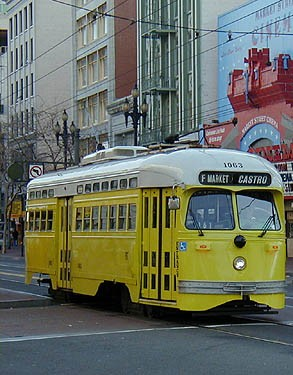
\includegraphics[width=.4\textwidth]{bus_left}} \quad 
	\subfloat[Right bus image]{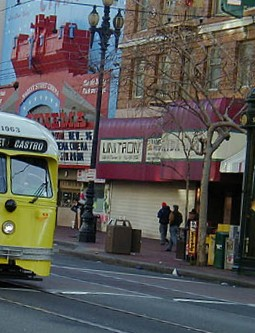
\includegraphics[width=.4\textwidth]{bus_right}}\\
	\subfloat[Matches between the images]{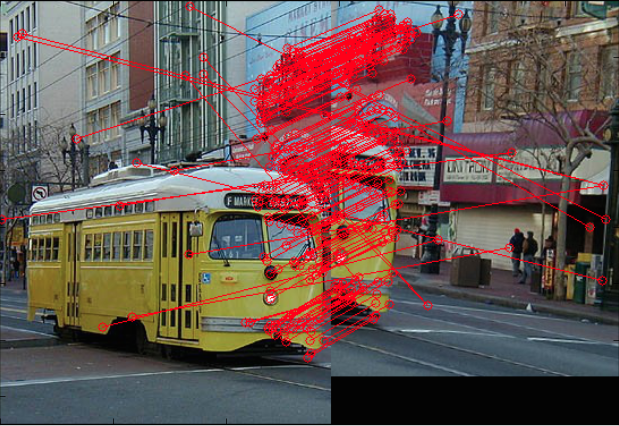
\includegraphics[width=.4\textwidth]{bus_matches}} \quad
	\subfloat[The two bus images stitched together]{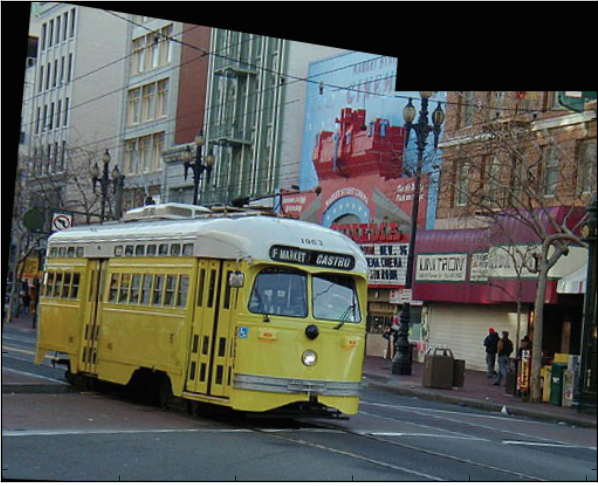
\includegraphics[width=.4\textwidth]{bus_stitched}} 
	\caption{The red lines between the images are the matches that are found. They can be used to find a transform that will have the last images as the result if the image are combined after transforming.}
	\label{fig:bus}
\end{figure}
